\documentclass[11pt]{scrartcl}

\usepackage[hidelinks, colorlinks=true]{hyperref}

\usepackage[english]{babel}
\usepackage{helvet}
\usepackage{mathpazo}
\usepackage{euler}
\usepackage{scrlayer-scrpage}
\usepackage[authoryear]{natbib}
\usepackage{csquotes}
\usepackage[normalem]{ulem}
\usepackage{xcolor}
\definecolor{@darkblue}{RGB}{0,0,140}
\definecolor{@darkgreen}{RGB}{0,100,70}
\definecolor{@darkred}{RGB}{140,5,5}
\hypersetup{
	colorlinks   = true, %Colours links instead of ugly boxes
	urlcolor     = @darkblue, %Colour for external hyperlinks
	linkcolor    = @darkblue, %Colour of internal links
	citecolor    = @darkgreen %Colour of citations
}
\usepackage[all]{hypcap}
\usepackage{subcaption}

\usepackage{amsmath}
\usepackage{amsfonts}
\usepackage{amssymb}
\usepackage{adjustbox}

\usepackage{float}
\usepackage{mathtools}
\usepackage{epigraph}
\usepackage{setspace}
\usepackage{listings}
\usepackage{algorithm}
\usepackage{algpseudocode}

\usepackage{tikz, pgfplots}
\usetikzlibrary{calc,decorations.pathmorphing,patterns, pgfplots.colorbrewer, shapes, arrows}
% Define block styles
\tikzstyle{decision} = [diamond, draw, fill=blue!20, 
text width=4.5em, text badly centered, node distance=3cm, inner sep=0pt]
\tikzstyle{block} = [rectangle, draw, fill=blue!20, 
text width=6em, text centered, rounded corners, minimum height=4em]
\tikzstyle{cheap} = [rectangle,  
text width=12em, text centered, minimum height=4em, node distance=3cm]
\tikzstyle{line} = [draw, -latex']
\tikzstyle{cloud} = [draw, ellipse,fill=red!20, node distance=3cm,
minimum height=2em]

\bibliographystyle{unsrt}

% ----------------- Layout stuff  -------------------------------

\pagestyle{scrheadings}
\clearscrheadfoot
%\automark{section}
%\renewcommand\sectionmark[1]{\markright{\MakeMarkcase {\thesection\hskip .5em\relax#1}}\rohead{\ifnum\expandafter\pdfstrcmp\botmark=0 \rightmark\else\leftmark{} --- \rightmark\fi}}


\ofoot{\pagemark}

% ---------------------  Title page setup ----------------------------
% Title Page
\title{Minimal Surfaces}
\author{Chenfei Fan \quad 390189 \\  Praveen Mishra\quad 389850 \\ Sankarasubramanian Ragunathan\quad 389851\\ Philipp Schleich\quad 391779}
%
\subject{Report \\ Simulation Sciences Laboratory}
\date{\today \\ \vspace{0.9cm}}

\publishers{
	\vspace{2em}
	
	\begin{tabular}[!b]{ll}
		Supervisor: & Prof. Dr. Uwe Naumann \\[3pt]
		            & Klaus Leppkes
	\end{tabular}
%	\begin{figure}[h!]
%		\centering
%		\includegraphics[width=.6\linewidth]{figs/mathccesText.png}%
%		
%	\end{figure}
}
% -------------------------------------------------------------

\newcommand{\mSurf}[1]{\ensuremath{\mathcal{F}\left[#1\right]}}
\newcommand{\mSurfDisc}[1]{\ensuremath{\mathtt{F}^h\left[#1\right]}}
\newcommand{\Dx}[1]{\ensuremath{\mathtt{d}_x[#1]}}
\newcommand{\Dy}[1]{\ensuremath{\mathtt{d}_y[#1]}}
\newcommand{\Dxx}[1]{\ensuremath{\mathtt{d}_{xx}[#1]}}
\newcommand{\Dyy}[1]{\ensuremath{\mathtt{d}_{yy}[#1]}}
\newcommand{\Dxy}[1]{\ensuremath{\mathtt{d}_{xy}[#1]}}

\newcommand{\inv}{\ensuremath{^{-1}}}
\newcommand{\vect}[1]{\boldsymbol{#1}}
\newcommand{\rb}[1]{\left( #1 \right)}
\newcommand{\cb}[1]{\left \{ #1 \right \}}

\begin{document}
\maketitle

%\section*{Abstract}
%\begin{abstract}
%\noindent Abstract might be unnecessary
%\end{abstract}
%
\clearpage
\protect \tableofcontents



\newpage
	
\onehalfspacing
% #########################################################################
\section{Introduction}
This report concludes our SiSc Laboratory Project in WS19/20, with the goal, to implement a software, that is able to numerically compute so called \emph{Minimal Surfaces}. As one might intuitively think, when we speak about surfaces, minimal has something to do with its surface. To this end, we define a \emph{Minimal Surface} to be a surface that locally minimizes its area (that is, the surface has a zero mean curvature over its domain). A trivial example is given by a plane. \cite{wiki:minsurf}

\begin{figure}[H]
	\centering
	\includegraphics[width=0.5\linewidth]{./figs/minsurfIntro.png}
	\caption{A surface with the local area vector.\\ For this surface to be minimal, $\lVert d\mathbf{A} \rVert \to \min $}
\end{figure}

Minimal surfaces appear in nature as well as they have some applications in engineering, while they can be observed both in macro- and microscopic length scale.
\begin{itemize}
	\item Macroscopic scale:
	\begin{itemize}
		\item Architectural design: Designing structures as minimal surfaces 
		\item Soap bubbles and dew drops
		\item Relativistic description of black holes
	\end{itemize}
	\item Microscopic scale:
	\begin{itemize}
		\item Material lattice structure
		\item Hydrophobic co-polymer structures
		\item Butterfly wings
	\end{itemize} 
\end{itemize}
\begin{figure}
	\vspace{-40pt}
	\centering
	\begin{subfigure}{.4\linewidth}
	\centering	
		\includegraphics[width=\linewidth]{./figs/BioGyroid.jpg}
		\caption{\scriptsize \cite[Gyroid minimal surface]{gan_biomimetic_2016}}\label{fig:111}
	\end{subfigure}
\hfill
	\begin{subfigure}{.4\linewidth}
	\centering
		\includegraphics[width=\linewidth]{./figs/Architecture.jpg}
		\caption{\scriptsize The West German pavilion, designed by Frei Otto.\cite{noauthor_frei_nodate}}\label{fig:222}
	\end{subfigure}
\end{figure}
Structures whose geometry makes up a minimal surface typically have large tensile strength, which can be used e.g. for man-made lightweight design in civil engineering (cf. figure~\ref{fig:111}) or lightweight design given by evolution, such as butterfly wings (gyroids, cf. figure~\ref{fig:222}. MSE is also used to provide a relativistic description on the formation of Black Holes. Material lattice structures of biological organisms such as butterfly wings are minimal surface structures ). Hydrophobic co-polymer structures also take the shape of a minimal surface in order to reduce the energy of the structure arising due to surface tension. \cite{gan_biomimetic_2016, wiki:minsurf}
% #########################################################################
\section{Background}
\subsection{Mathematical basics}\label{sec:mathbasics}
We look at surfaces in $ \mathbb{R}^3 $, defined over an open set $\Omega \subset \mathbb{R}^2$. 
The surface of desire should contain the least possible area among all possible surfaces, that assume given values on the boundary of $\Omega$, denoted by $\partial \Omega$. \cite{Sakai1976}

Lagrange showed in 1760, that such a surface is characterized by the graphic of a function $z(x,y)$, $z: \mathbb{R}^2 \to \mathbb{R} $, which is twice continuously differentiable on a two-dimensional domain, particularly in a subset of $\mathbb{R}^2$.
This function $z$ has to fulfill the so called \textit{Minimal-Surface Equation} (MSE) stated below.
\begin{align}\label{eq:MSE}
	(1+z_y^2) z_{xx} - 2 z_x z_y z_{xy} + (1+z_x^2)z_{yy} = \mSurf{z} &= 0 \quad &\text{in } \Omega \\
	z(x,y) &= g(x,y) \quad &\text{on } \partial \Omega \notag
\end{align}
Clearly, this formulation satisfies the prescribed boundary values given by $g(x,y)$ due to the Dirichlet boundary condition on $\partial\Omega$.
As to why the graphic of functions solving this equation describes a minimal surface, we refer to the literature. For example \cite{Sakai1976} gives a very straightforward proof.

In the following, we will call the differential operator $\mSurf{\cdot}$ the Minimal-Surface Operator (MSO). The resulting partial differential equation (PDE) in eq. \eqref{eq:MSE} turns out to be an elliptic PDE of second order, which is in particular \textit{non-linear}. The solution of such a PDE is not trivial, and typically requires numerical treatment. For certain cases, analytical descriptions are available, such as for Scherk's surface.

\begin{figure}
	\centering
	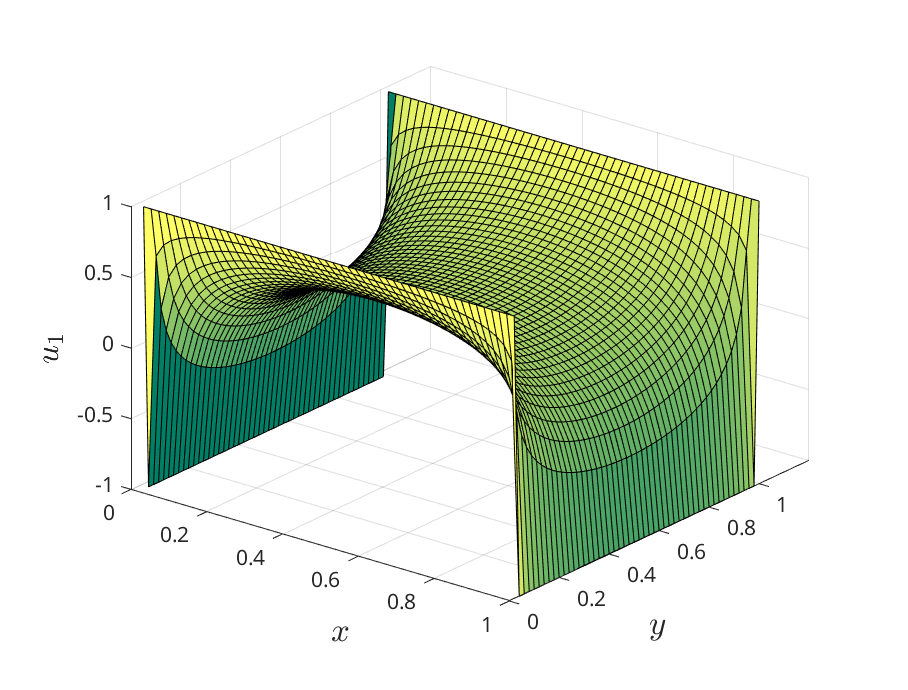
\includegraphics[width=.5\textwidth]{figs/scherk-test}
	\caption{Scherk's first surface on $[0,1]^2$}\label{fig:scherk01}
\end{figure}


\newpage

As an example, Scherk's first surface (compare to figure \ref{fig:scherk01}) $\Sigma$ rescaled on $\Omega = [0,1]^2$ is given by
\begin{equation}
	\Sigma = \left\{ \left. \left(x, y, \log \left( \frac{\cos (\pi(x-\frac{1}{2}))}{\cos (\pi(y-\frac{1}{2}))} \right) \right) \in \mathbb{R}^{3} \right  | 0 < x, y < 1 \right\}.
\end{equation} 
which is the limit $n\to \infty$ of 
\begin{align}
\Sigma_n = \left\{ \left. \left(x, y, u_n(x,y) \right) \in \mathbb{R}^{3} \right  | 0 < x, y < 1 \right\}, \\
\lim\limits_{y\to \pm 1} \to n \quad, 0 \le x \le 1 \\
\lim\limits_{x\to \pm 1} \to -n \quad, 0 \le y \le 1.
\end{align}
\cite{wiki:scherk}

The numerical solution of the MSE will require setting approbiate boundary conditions. Since $\log \left( \frac{\cos (\pi(x-\frac{1}{2}))}{\cos (\pi(y-\frac{1}{2}))} \right) \to \pm \infty $ on $\partial\Omega$, this is numerically not very practical. 

We thus introduce $\beta_x,\beta_y \in (0,1)$ s.th. 
\begin{equation}
\Sigma_{\text{trunc}} = \left\{ \left. \left(x, y, \log \left( \frac{\cos (\pi\beta_x(x-\frac{1}{2}))}{\cos (\pi\beta_y(y-\frac{1}{2}))} \right) \right) \in \mathbb{R}^{3} \right  | 0 < x, y < 1 \right\}.
\end{equation} 

By these means, we solve the MSE on $\Omega_\text{trunc}=[0,1]^2\subset\Omega$ with $\Omega=[0,\frac{1}{\beta_x}]\times[0,\frac{1}{\beta_y}]$. Exact boundary values on $\partial\Omega_\text{trunc}$ ensure the correctness of the results. We choose $\beta_x=\beta_y=\beta$, as we restrict ourselves to solving on a square domain.

Later on, we will use this surface as a test-case to verify our numerical results.

\newpage
\subsection{Numerical solution}
\subsubsection{Discretization}
\label{section:Discretization}
In this project, we are supposed to solve the MSE numerically on $\Omega \equiv (0,1)\times(0,1)$. In the following, discretized quantities are indicated by a superscript $h$. The spatial domain is to be discretized using a structured mesh with equidistant grid spacing both in $x,y$, i.e. we have the same number of grid points in both directions, $N=N_x=N_y$. Thus, we define $\Omega^h := \{ (x,y) \in \mathbb{R}^2:\text{ }(x,y) = (ih, jh), \text{ } 0 \le i,j < N,\text{ }hN=1\}$.

\begin{figure}[h!]
	\centering
	\adjustbox{scale=3}{ 
	\begin{tikzpicture}
	\draw [gray!50!white, step=0.2] (-0.3,-0.3) grid (1.3,1.3);
	\draw [thick, ->] (0,-0.4) -- (0,1.4);
	\draw [thick, ->] (-0.4,0) -- (1.4,0);
	
	\draw [red, thick] (0,0) rectangle (1,1);
	
	\node at (-0.17,-0.14) [scale=0.4] {(0,0)};		
	\node at (1.17,-0.14) [scale=0.4] {(1,0)};		
	\node at (-0.17,1.1) [scale=0.4] {(0,1)};		
	\node at (1.17,1.1) [scale=0.4] {(1,1)};	
	\node at (-.55, .7) [blue, scale=.5] {$\Omega^h$};	
	\node at (-.4, .45) [red, scale=.5] {$\partial\Omega^h$};	
	
	
	
	% Boundary nodes
	\foreach \x in {0,1,2,3,4,5} {
		\foreach \y in {0} { % bottom
			\node at (\x/5,\y/5) [circle,fill=red, scale=0.3] {};
			%this way circle of nodes will not be transformed
		}
	}
	\foreach \x in {0} { % left
		\foreach \y in {0, 1,2,3,4,5} {
			\node at (\x/5,\y/5) [circle,fill=red, scale=0.3] {};
			%this way circle of nodes will not be transformed
		}
	}
	\foreach \x in {0,1,2,3,4,5} { % top
		\foreach \y in {5} {
			\node at (\x/5,\y/5) [circle,fill=red, scale=0.3] {};
			%this way circle of nodes will not be transformed
		}
	}
	\foreach \x in {5} { % right
		\foreach \y in {0,1,2,3,4,5} {
			\node at (\x/5,\y/5) [circle,fill=red, scale=0.3] {};
			%this way circle of nodes will not be transformed
		}
	}
	%Inner nodes
	\foreach \x in {1,2,3,4} {
		\foreach \y in {1,2,3,4} {
			\node at (\x/5,\y/5) [circle,fill=blue, scale=0.3] {};
			%this way circle of nodes will not be transformed
		}
	}
	\end{tikzpicture}
	}
	\caption[Depiction of $\Omega^h$ with $N=5$, $hN=1$]{Depiction of $\Omega^h$ with $N=5$, $hN=1$. Blue: inner nodes, red: boundary nodes}
\end{figure}

We choose to discretize the MSO on $\Omega^h$ by Finite Differences, since this is usually the easiest way to go, and on a structured grid, would anyways yield similar discrete equation as in Finite Volume or Finite Element methods.

To obtain a second order consistent discrete MSO ($\mSurfDisc{\cdot}$), we use central difference stencils on the first, second and mixed derivative, assuming that the underlying solution is at least twice continuously differentiable. This can be perceived as a constraint on the boundary conditions that are set in the numerical solution: In case $g$ does not have sufficient regularity, convergence is not guaranteed. Since all these stencils have make only use of immediate neighours, there is no need to treat nodes close to the boundary differently, since the boundary is given by $g(\cdot)$.
\newpage 
This way, we obtain a discrete version of \eqref{eq:MSE}:
\begin{align}
	\left(1+\Dx{z^h}^2\right)\Dyy{z^h}-\Dx{z^h} \Dy{z^h}\Dxy{z^h} + \left(1+\Dy{z^h}^2\right)\Dxx{z^h} = \mSurfDisc{z^h} &= 0  \quad \text{in } \Omega^h \notag \\
	z^h &= g \quad \text{on } \partial\Omega^h \label{eq:dMSE},
\end{align}
while the stencils defined on the inner nodes are given as follows ($1 \le i,j \le N-1$):
\begin{align}
	\Dx{z}_{i,j} &= \frac{z_{i+1,j}-z_{i-1,j}}{2h}\label{eq:dx} \\
	\Dy{z}_{i,j} &= \frac{z_{i,j+1}-z_{i,j-1}}{2h}\label{eq:dy} \\
	\Dxx{z}_{i,j} &= \frac{z_{i+1,j} - 2z_{i,j} + z_{i-1,j}}{h^2}\label{eq:dxx}\\
	\Dyy{z}_{i,j} &= \frac{z_{i,j+1} - 2z_{i,j} + z_{i,j-1}}{h^2}\label{eq:dyy}\\
	\Dxy{z}_{i,j} &= \frac{z_{i+1,j+1} + z_{i-1,j-1} - z_{i-1,j+1}-z_{i+1,j-1}}{4h^2}\label{eq:dxy}. 
\end{align}
Figure~\ref{fig:fdmmesh} depicts the stencils on a segment of $\Omega^h$.
Since the stencils have only support to the nearest neighbors, there is no need tho treat nodes close to the boundary any different. Furthermore, this gives already rise to the conclusion, that the associated matrix will be sparse (for each of the $N$ gridpoints, only 9 instead of $N$ partners contribute).

\begin{figure}
	\centering
	\includegraphics[width=.4\linewidth]{figs/FDMMesh}
	\caption{Snippet of the mesh with Finite Differences stencils\\red/blue: first and second order stencils in $x,y$\\
	green: mixed stencil}\label{fig:fdmmesh}
\end{figure}
\newpage
\subsubsection{Solution}
The main difficulty in solving the MSE lies in the non-linearity of $\mSurfDisc{\cdot}$. Since it is not possible, to directly invert for $z^h = \left(\mathtt{F}^h\right)\inv 0$, one needs to use a procedure such as Newton-Raphson iterations. The main idea is to use some initial guess $z^h_0$, while in general, $\mSurfDisc{z^h_0}=r^h_k\neq0$. The goal is then to generate a sequence of $z^h_k$ such that $r^h_k\to 0$ for increasing, but reasonably small $k$. Algorithm~\ref{algo:standard-newton} shows the standard Newton-Raphson procedure, that takes as input a specific initial guess (here: 0), a tolerance for convergence \textsc{tol} and the nonlinear operator $\mSurfDisc{\cdot}$, outputting an approximate solution to the MSE $z^h_{k_\text{fin}}$.
\begin{algorithm}
	\caption{Newton's method applied on the discrete MSE}\label{algo:standard-newton}
	\begin{algorithmic}
		\State $k \gets 0$ 
		\State $z^h_k \gets 0 $ 
		\State $r^h_k \gets \mSurfDisc{z^h_k}$
		\While{$\lVert r^h_k \rVert > \textsc{tol}$} \Comment{ We choose $ \lVert \cdot \rVert = \lVert \cdot \rVert_2  $}
			\State $z^h_{k+1} \gets z^h_{k} - \left(\nabla\mSurfDisc{z^h_k}\right)\inv r^h_k $
			\State $k \gets k+1$ 
			\State $r^h_k \gets \mSurfDisc{z^h_k}$
		\EndWhile
	\end{algorithmic}
\end{algorithm}

This algorithm involves the computation of the inverse of the gradient of $\mSurfDisc{z^h_k}$ for each iteration $k$. Later, we will present and compare two different ways on how to contrive this.

It is well known, that the Newton-Raphson procedure yields fast convergence, but the success of this convergence is highly dependent on the initial guess $z^h_0$. Furthermore, convergence can be improved by choosing an initial guess that is closer to the solution. 
One possible initial guess is to take the average boundary value, \\$z^h_{0,\text{ave}}=\frac{1}{|\partial\Omega^h|} \sum_{(x_i,y_j)\in \partial\Omega^h} \big(g(x_i,y_j)\big)$. While this might help convergence for surfaces, that have a certain offset with respect to the $x,y$-plane, it does not provide any additional information (such as preshaping the correct curvature).

To obtain a more educated initial guess, recall the MSE, equation \eqref{eq:MSE}. Considering only linear terms, we get 
\begin{align}
	\mathcal{L} [z] = z_{xx} + z_{yy} &= 0 \quad\quad\quad\quad \text{ in } \Omega \\
	z(x,y) &= g(x,y) \quad \text{ on } \partial\Omega \notag 
\end{align}\newpage
This linear, second order PDE is well known as the Laplace-equation, and can be solved by discretizing the second derivatives using the definitions for $\Dxx{\cdot},\Dyy{\cdot}$ introduced before, yielding $\mathtt{L}[z^h]=0 $ with the usual boundary conditions. Since Laplace's equation can be regarded as a linearization of the MSE, we suspect to get a better initial guess (and thus faster and a more robust convergence behaviour) by first solving for $z^h_0= \mathtt{L}\inv 0$. This way, we obtain a slightly modified version of Algorithm~\ref{algo:standard-newton}, stated in Algorithm~\ref{algo:laplace-newton}.

\begin{algorithm}
	\caption{Newton's method using Laplace's Equ. as initial guess}\label{algo:laplace-newton}
	\begin{algorithmic}
		\State $k \gets 0$ 
		\State $z^h_k \gets \mathtt{L}\inv 0 $ \Comment{Solve Laplace's Equ. as initial guess}
		\State $r^h_k \gets \mSurfDisc{z^h_k}$
		\While{$\lVert r^h_k \rVert > \textsc{tol}$} 
		\State $z^h_{k+1} \gets z^h_{k} - \left(\nabla\mSurfDisc{z^h_k}\right)\inv r^h_k $
		\State $k \gets k+1$ 
		\State $r^h_k \gets \mSurfDisc{z^h_k}$
		\EndWhile
	\end{algorithmic}
\end{algorithm}

\clearpage
\subsection{Consequences for a implementation}
So far we discussed the abstract numerical setting to solve the MSE. But when implementing this as a software solution, one has to consider several additional points, which especially involve the interface to the user.

We provide an overview of requirements for a potential implementation in figure~\ref{fig:requs}.

\begin{figure}[b]
	\centering
	\begin{tikzpicture}[node distance=4cm, auto]
	% Place nodes
	\node [block] (code) {Code/Solver};
	\node [cloud, left of=code, node distance=3cm] (in) {user input};
	\node [cloud, right of=code, node distance=3.5cm] (out) {output to user};
	%
	\path [line] (in) -- (code);
	\path [line] (code) -- (out);
	
	\node [cheap, below of=in](inputLegend) at(-3.95,0.3) {
		\small\begin{itemize}
		\item mesh size 
		\item boundary conditions 
		\item various tuning parameters
		\end{itemize}
		$\rightarrow$ user interface \\ via input file \normalsize
	};
	
	\node [cheap, below of=code] (solverLegend) at(0,0.25) {%
		\small\begin{itemize}
		\item discretization/grid 
		\item apply BC 
		\item determine Jacobian 
		\item solve linear systems 
		\item Newton iterations  \normalsize
		\end{itemize}
	};
	
	\node [cheap, below of = out] (outLegend) at(3.8, 0.3) {
		\small\begin{itemize}
		\item visualization of solution 
		\item convergence output (residual) 
		\item check validity of result
		\end{itemize}\normalsize
	};
	\end{tikzpicture}
	\caption{Requirements on a potential implementation}\label{fig:requs}
\end{figure}
We can divide communication with the user into user input and output to the user. A input interface can be realized e.g. as a GUI (graphical user interface) or as a input file (text file, that is parsed before/while running the simulations). Either realization serves the purpose to give the user a convenient possibility to set the main simulation parameters such as grid size and boundary conditions, as well as to set several tuning parameters like number of threads for parallel execution, initial guess.

The output to the user further is crucial in the sense that without giving the user any opportunity to perceive the result of the computation, there is no point in even computing anything. In terms of our application, it is required to provide the result in a form that can easily be visualized as a 3D-object. Additionally, one might want to offer a convenient validity-check and information about convergence.

Last but not least, a software implementation also needs to be able to perform all of the key steps to solve the MSE: It must allow for a discretizaion of the computational domain, and for setting the desired values on its boundary. Apart from implementing a suitable initial guess, inside a loop such as Algorithms~\ref{algo:standard-newton},~\ref{algo:laplace-newton} there are a few important tasks missing that require special consideration: Both computing the Jacobian $\nabla\mSurfDisc{\cdot}$ and solving the resulting linear systems are non-trivial necessities whose treatment will be discussed in more detail in the next chapter. 


\clearpage
% #########################################################################
\section{Implementation}
%##########################################################################
\subsection{Software/Solver Design}
In order to meet the requirements, that have been identified earlier, we create four different classes. These classes are individually responsible for a certain subset of tasks. 

A user interface will be given by a input file, called \texttt{params.in}, which is parsed by the class \texttt{inputparser}. Creating an object of \texttt{inputParser} thus allows us to access the input file from any other place in the code. Further, \texttt{cartesianGrid} takes care of the discretization, and an instance of such a grid enables to access the specifics of our equidistant, square mesh. The most important part of our code is made up by the class \texttt{solver}, which contains all required numerical (sub-)routines. Last but not least, the \texttt{postProcessor}-class builds the connection to the user after having completed a simulation, providing information about solution and convergence.
  
\begin{figure}[H]
	\includegraphics[width=\textwidth]{./figs/ReportUML.pdf}
	\caption{UML Diagram with the strucuture of the \textit{minSurf} software.}
	\label{fig:UMLDiag}
\end{figure}
\newpage
Figure \ref{fig:UMLDiag} shows the structure of the software, the classes and their associated functions, developed in order to solve the minimal surface problem. In the following, the individual classes are again described in more detail.
\begin{itemize}
	\item {\texttt{inputParser:} This class consists of functions necessary to read all the parameters required to control and execute the minimal surface software. This class takes in \texttt{params.in} which contains all the necessary parameters such as the number of mesh elements\footnote{represented by $N$, the number of elements per dimension}, boundary conditions, option for the method of Jacobian computation, etc. as an input to be parsed and processed. This class also depends on an external library, \texttt{ATMSP Expression Parser}\footnote{We modified this parser slightly, such that it is also able to parse piece-wise boundary conditions. The original library is available at \url{https://sourceforge.net/projects/atmsp/}}, to parse the boundary conditions.}
	\item {\texttt{cartesianGrid:} This class consists of functions that help in the generation of a uniform cartesian mesh required for solving the Finite Difference discretization. It also has functions able to return the $x$ and $y$ coordinates of a node required to apply the boundary conditions. Moreover, it provides methods to allocate separate storage of boundary and inner node indices.}
	\item {\texttt{solver:} This class consists of functions required to solve the minimal surface problem using Newton-Raphson method. The function to apply the boundary conditions is specified inside this class. \texttt{ATMSP Expression Parser} library is again required for this as the library provides methods to parse the boundary condition given as a string expression inside \texttt{params.in} into an executable byte code. It also uses \texttt{DCO} library to compute the Jacobian required for the  Newton Raphson iterations. Separate function definitions are created to run the solver for different options of Jacobian such as Symbolic differentiation, AD by Hand and Matrix-free methods based on the option provided inside \texttt{params.in}}
	\item  {\texttt{postProcessor:} This class contains functions designed to write the solver residual as a CSV file and the resulting minimal surface as a VTS file allowing 3D visualization using \textit{Paraview}. To write the VTS file, the class uses the \texttt{VTK} library. It also provides a function to compare the convergence of the numerical towards the analytical solution for the special case of the Scherk surface. The error is measured using both the  maximum-norm ($\lVert z-z^h \rVert_\infty := \max\limits_{1\le i,j\le N} \lvert z_{ij}-z^h_{ij}\rvert$ ) as well as the  $\ell_2$-norm ($\lVert z-z^h \rVert_2 := \sqrt{ \frac{1}{N^2} \sum_{i,j=1}^{N} \big(z_{ij}-z_{ij}^h\big)^2}$).}
\end{itemize}
%##########################################################################
\subsection[A note on solving linear systems]{A note on solving linear systems (does not affect the matrix-free solver)}
When solving the MSE, we deal in general with sparse, non-symmetric systems. The \texttt{Eigen} library (we use the release Eigen 3.3.7) provides the following sparse linear algebra methods\footnote{Due to the severe sparsity of the matrix, we did not consider a dense matrix implementation.}, that would be suitable for our problem:
\begin{itemize}
	\item SparseLU -- a sparse version of LU-decomposition 
	\item BiCGSTAB -- Stabilized biconjugate gradient descent (more costly than CG, but suitable for general square matrices). Essentially, this represents a CG-routine inside GMRES(1)
	\item GMRES -- Generalized Minimum Residual Method 
\end{itemize}
The latter two are linear iterative schemes suitable for general matrices, while we exclude GMRES from now on, as BiCGSTAB is slightly more efficient according to benchmarks of the \texttt{Eigen} library\footnote{\url{http://eigen.tuxfamily.org/dox/group__TopicSparseSystems.html}, in the very bottom, assuming both use the ILUT preconditioner}. In contrast to LU decomposition, which is a direct method, linear iterative schemes might be faster, but do not guarantee convergence. This depends on the system to be solved. As it turns out, the MSE using Finite Differences yields sufficiently well behaved systems, that typically converge.

The convergence of iterative schemes can be (dependent on the system) boosted by the use of preconditioners. In \texttt{Eigen}, either the identity, a Jacobi (diagonal, iff non-zero) or a incomplete LU-decomposition (ILUT) preconditioner are available, while the latter in general has the most potential to speed up convergence. 

Testing these methods on our initial-guess subroutine, which solves the Laplace-equation, has yielded, that, while SparseLU is faster than BiCGSTAB+Jacobi, the right tuning of ILUT in combination with BiCGSTAB is fastest. 

Still though, our implementation inside the Newton-iteration uses bare BiCGSTAB with Jacobi-preconditioner. The reason therefore is, that we chose to represent the discrete system not as the reduced system (i.e. boundary information is brought onto the right-hand-side, yielding a system size of $(N-2)^2$ instead of $N^2$), but as the full system\footnote{We discussed this with our supervisor in the beginning of the project, and concluded that solving the full system would not have substantial drawbacks and would be more intuitive to implement.}. While this has no impact on the feasibility of a LU-decomposition when solving the Laplace-equation, it prohibits a LU-decomposition on the full system. 

Solving the Laplace-equation can be done in one step -- this means, we prescribe the boundary information by putting the associated values on the right-hand-side, and insert an (almost) empty row\footnote{With empty row, we mean a row, that is only made up by 0-elements.}, that carries a 1 on the place, that is to be multiplied with the boundary value at its respective position. In conclusion, the system matrix, that is to be inverted, has still full rank $\Leftrightarrow$ does not contain an empty row. What changes now for the linear systems inside the Newton iterations? We start with an initial guess $z^{(0)}$, which already must contain the boundary information. The linear systems arise, when we want to get from $z^{(i)}$ to $z^{(i+1)}$ -- the difference $dz^{(i)}$ resulting from the linear solve must not change the boundary information, since both  $z^{(i)}$ and $z^{(i+1)}$ inherit already the correct values from $z^{(0)}$. As a consequence the Jacobian of the MSO $\nabla\mSurfDisc{z^{(i)}}$ has an empty row, whenever the row index corresponds to a boundary node. This would prevent us from using SparseLU or an iterative scheme with the ILUT preconditioner. BiCGSTAB+Identity still works, since it only relies on matrix-vector products and scalar products, and multiplying empty rows is not forbidden (but unnecessary work)\footnote{Jacobi preconditioner also can be used, since it only acts if the diagonal entry is non-zero}.

We can overcome this by putting some little extra effort, and setting a 1-entry on the diagonal of the Jacobian of the discrete MSO, if the row corresponds ot a boundary index. This does not change the result, since we are exact on the boundary for all iterations, thus the right-hand-side in this case is 0. By such a procedure, we end up with a non-singular Jacobian, and can use direct methods and preconditioners. As before, numerical tests suggest that for the right tuning, BiCGSTAB+ILUT is the fastest option for our problem, while SparseLU would be still faster that BiCGSTAB+Jacobi. 
Next, note, that the Newton procedure does not require the 'exact' value of $dz^{(i)}$, but can be satisfied with a solution up to a certain tolerance\footnote{keyword in \texttt{params.in}: $\textsc{tol}_\text{linsolver}$}, on one hand enables us to choose this tolerance of the same order\footnote{in some cases even slightly larger -- this requires possibly more iterations, while each linear solve is less and less costly}. This allows us to additionally boost the runtime of the iterations by choosing a smart value for this linear solve tolerance. 

Therefore, we choose this to be the default in our solver. We are not providing a switch option to change the solver, because the software is only capable of solving this very PDE, which means we do not have to expect a substantially different structure of the Jacobian\footnote{Depending on boundary conditions, it has different entries, but the non-zero pattern stays the same in general.}. Apart from that, as stated before, the iterative scheme does not rely on exact updates, which can only be exploited using iterative schemes. Therefore, a single, but optimal, solver option shall be sufficient. 


\subsection{Computing the Jacobian}
Within the Newton iterations, it is necessary to compute the inverse of the Jacobian of the discrete MSO and solve the resulting linear systems. One well-known approach is using Finite Differences to further discretise the discrete MSO, but it is not efficient when the mesh is very fine. As a result, Algorithmic Differentiation is used in this problem. We implemented this procedure following two different strategies:
\begin{itemize}
	\item Build the Jacobian by Algorithmic Differentiation (AD by hand) and compute its inverse by existing linear solvers.
	\item Do not explicitly build the Jacobian, but use existing AD libraries to extract its action on certain vectors. Substitute this into the self-implemented matrix-free linear solver.
\end{itemize}
To get an overview of the problem's dimensions and properties as well as to provide a solution to verify other approaches based on Algorithmic Differentiation, we first implemented a straightforward ("hard-coded") method to derive the required Jacobian $\nabla \mathtt{F}(z)$ by substituting Equ.~\eqref{eq:dx}-\eqref{eq:dxy} into Equ.~\eqref{eq:dMSE} and taking its derivatives of $\vect{z}$. As is indicated in section~\ref{section:Discretization}, the resulting Jacobian is sparse, so it is stored in \texttt{Eigen::SparseMatrix} format by \texttt{Eigen} library. Then solve $dz = \nabla\mSurfDisc{z^h_k}\inv y$ by Biconjugate gradient stabilized method (BiCGSTAB). It is used instead of BiCG or CG since $\nabla\mSurfDisc{z^h_k}$ is not symmetric in general.

\subsubsection{AD by hand}
As is shown in section~\ref{section:Discretization}, the discrete MSO of each gridpoint has only support from its 9 neighbors. Considering the derivation of the Jacobian as a loop of gridpoint-wise MSO over each gridpoint (which is parallelizable in nature), the gridpoint-wise discrete MSO for each gridpoint $(i,j)$ can be generalized as Equ.~\eqref{eq:mso}, where $h$ is a function which has 1 output $\mathtt{F}\rb{z[i][j]}$ and 9 inputs $z[i'][j'], i'\in\{i, i\pm1\}, j'\in\{j,j\pm1\}$. Given this function primal of $ \mathtt{F}: \mathbb{R}^n\rightarrow 1 $ (here $n=9$), it is advantageous to use a first-order adjoint model as Equ.~\eqref{eq:adj1}, \eqref{eq:adj2}. By seeding the output $y_{(1)}$ one can harvest the whole Jacobian row-wise, where one row of the Jacobian has only 9 non-zero entries. The function signature of the overloaded function is stated in Equ.~\eqref{eq:adj}. By the driver function in Equ.~\eqref{eq:adj.driver} (assume an inner gridpoint $(i,j)$ has index $idx$), one column of the Jacobian $a1\_z[idx][:]$ together with the primal $z[idx]$ is harvested for each gridpoint $(i,j)$.

\begin{equation}
\mathtt{F}\rb{z[i][j]} = h\rb{z[i'][j'], i'\in\{i, i\pm1\}, j'\in\{j,j\pm1\}}\label{eq:mso}
\end{equation}

\begin{align}
y &:= \mathtt{F}(\textbf{x})\label{eq:adj1} &&
\\
\textbf{x}_{(1)} &:= \nabla \mathtt{F}(\textbf{x})^{T} \cdot y_{(1)}\label{eq:adj2}
\end{align}

\begin{equation}
\rb{y, \textbf{x}_{(1)}} := \mathtt{F}_{(1)}\rb{\textbf{x}, y_{(1)}}\qquad \mathtt{F}_{(1)}: \rb{\mathbb{R}^n\times 1}\rightarrow \rb{1\times\mathbb{R}^n}\label{eq:adj}
\end{equation}

\begin{equation}
\rb{z[idx],\ a1\_z[idx][:]} = \mathtt{F}\rb{z[:],\ a1\_Fz[idx]}
\label{eq:adj.driver}
\end{equation}

The row-wise derivation of the Jacobian inside a loop over all inner gridpoints can be decomposed into a single assignment code (SAC). Example of code snippets for each inner gridpoint if index $i$ are as Code~\ref{lst:prsac}, \ref{lst:adsac}. Because of the sparsity of the Jacobian, the computational complexity for each inner gridpoint is a constant. Therefore, the total computational complexity is $\mathcal{O}(N^2)$ for $N^2$ gridpoints (or to say, $N^2$ rows of the Jacobian).

Same as the "hard-coded" method, we store the derived Jacobian in \texttt{Eigen::SparseMatrix} format and solve the linear system by BiCGSTAB.

Results have proven that we apply Algorithmic Differentiation to the problem and get a feasible result. However, since it is "by hand", it has certain limitations. If the problem is more complex, it is inefficient, or even impossible to manually derive it step by step. A more general approach is still needed to automatically derive the Jacobian without manual computation.

\lstset{backgroundcolor=\color{gray!20}, language=C++, basicstyle=\ttfamily, breaklines=true}

\noindent
\begin{minipage}[t]{0.45\linewidth}
\begin{lstlisting}[caption={Adjoint SAC Code for inner gridpoint $i$ (primal/forward)},label=lst:prsac,language=C++]
// d(...) = fd(x)
dx = (z[i+1]-z[i-1])/(2*h);
dy = (z[i+N]-z[i-N])/(2*h);
dxx, dxy, dyy = ...

// intermidiates v1, v2, v3
v1 = (1+pow(dx,2))*dyy;
v2 = -2*dx*dy*dxy;
v3 = (1+pow(dy,2))*dxx;

// result
Fz[i] = v1+v2+v3;
\end{lstlisting}
\end{minipage}\hfill
\begin{minipage}[t]{0.53\linewidth}
\begin{lstlisting}[caption={Adjoint SAC Code for inner gridpoint $i$ (adjoint/reverse)},label=lst:adsac,language=C++]
(initialize everything to zero)
// seed a1_Fz
a1_Fz[i] = 1.0;

// result Fz[i] = v1+v2+v3
a1_v1 = a1_Fz[i];
a1_v2 = a1_Fz[i];
a1_v3 = a1_Fz[i];

// intermidiates v1, v2, v3
a1_dy = dxx*2*dy*a1_v3;
a1_dxx = (1+pow(dy,2))*a1_v3;
...

// d(...) = fd(x)
a1_z[i][i+1] = a1_dx/(2*h)+...;
a1_z[i][i-1] = a1_dx/(-2*h)+...;
...
\end{lstlisting}
\end{minipage}

\subsubsection{Matrix-free linear solver with \texttt{dco\_c++}}
\texttt{dco\_c++} is a library that implements Algorithmic Differentiation by overloading in C++. It provides the same function as AD by hand in terms of harvesting the Jacobian. However, if all manual computation is eliminated, it is unable to exploit the sparsity of the Jacobian, so we need $\mathcal{O}(N^4)$ space to store it, which for large $N$ is impossible. Therefore, we implemented a matrix-free linear solver inside Newton's method as described in Algorithm~\ref{algo:matfree-newton}, which does not require explicitly building the Jacobian, but instead apply the vector tangent code overloaded by \texttt{dco\_c++} as a matrix-vector multiplication tool which multiplies the Jacobian with the seed to harvest the result.

In general, the MSO is an operator of $ \mathtt{F}: \mathbb{R}^{N\times N}\rightarrow \mathbb{R}^{N\times N} $, which has the same computational complexity for vector tangent mode and vectors adjoint mode. We choose vector tangent mode in our implementation.

\begin{algorithm}[H]
	\caption{Newton's method}\label{algo:matfree-newton}
	\begin{algorithmic}
		\State $\vect{y} \gets \mathtt{F}(\vect{z})$ 
		\While{$\lVert \vect{y} \rVert > \textsc{tol}$} 
		\State $\vect{A} = \nabla \mathtt{F}(\vect{z})$ 
		\State \color{blue} $\vect{dz} = \vect{A}\inv \vect{y}$  \normalcolor \Comment{Instead of assembling the whole $\nabla \mathtt{F}$ above, do this matrix-free}
		\State $\vect{z} \gets \vect{z} + \vect{dz}$
		\State $\mathtt{res} \gets \mathtt{F}(\vect{z})$ 
		\EndWhile
	\end{algorithmic}
\end{algorithm}

The first-order vector tangent mode for $\mathtt{F}: \mathbb{R}^{N\times N}\rightarrow \mathbb{R}^{N\times N} $ is defined as Equ.~\eqref{eq:tg1}, \eqref{eq:tg2}, and its function signature is defined in Equ.~\eqref{eq:tg}. By substituting Equ.~\eqref{eq:tg1} into an existing linear solver (for example BiCGSTAB, as we implemented in Algorithm~\ref{algo:bicgstab}), $\vect{dz} = \vect{A}\inv \vect{y}$ is solved by this iterative approach.

The advantage of the matrix-free linear solver with \texttt{dco\_c++} is that it does not require any prior knowledge of the operator. Given any primal \texttt{y = F(z)} where $ \mathtt{F}: \mathbb{R}^{N\times N}\rightarrow \mathbb{R}^{N\times N} $, only several lines of code is needed for the vector tangent mode by overloading, as is shown in Code~\ref{lst:vot}.
\begin{lstlisting}[caption={Vectors of Tangents by Overloading},label=lst:vot,language=C++]
// activate
std::vector<ADtype> z_(std::begin(z),std::end(z));
// seed
for (auto& i: grid.innerNodeList) 
dco::derivative(z_)[i] = dz[i];
// compute
y_ = F(z_); // overloaded
// harvest
dy = dco::derivative(y_);
\end{lstlisting}

\begin{align}
\textbf{y} &:= \mathtt{F}(\textbf{x})\label{eq:tg1} &&
\\
Y^{(1)} &:= \nabla \mathtt{F}(\textbf{x}) \cdot X^{(1)}\label{eq:tg2}
\end{align}
\begin{equation}
\rb{\textbf{y}, Y^{(1)}} := \mathtt{F}^{(1)}\rb{\textbf{x}, X^{(1)}}\qquad \mathtt{F}^{(1)}: \rb{\mathbb{R}^{N\times N}\times \mathbb{R}^{N\times N}}\rightarrow \rb{\mathbb{R}^{N\times N}\times\mathbb{R}^{N\times N}}\label{eq:tg}
\end{equation}

\begin{algorithm}[H]
	\caption{Matrix-free BiCGSTAB to get $\vect{dz}$ (adapted from \cite{naumann})}\label{algo:bicgstab}
	\small{	\begin{algorithmic}
			\State $\vect{z}^{(1)} \gets \vect{dz}$ 
			\State \color{blue}$(\vect{y}, \vect{y}^{(1)}) \gets \mathtt{F}^{(1)} (\vect{z}, \vect{z}^{(1)}) $ \normalcolor \Comment{DCO}
			\State $\vect{p} \gets -\vect{y} -\vect{y}^{(1)}$
			\State $\vect{r} \gets \vect{p}, \vect{r_0}\gets \vect{r},\vect{p}\gets \vect{0},\vect{v}\gets \vect{0}, \rho\gets1,\alpha\gets1,\omega\gets1 $
			\While{$\lVert \vect{r} \rVert > \textsc{tol}$} 
			\State $\rho_{\text{new}} = \big(\vect{r_0},\vect{r}\big)$
			\State $\beta \gets \rho_{\text{new}}/\rho \cdot \alpha/\omega$
			\State $\rho \gets \rho_{\text{new}}$
			\State $\vect{p}\gets \vect{r}+\beta(\vect{p}-\omega \vect{v})$
			\State $\vect{z}^{(1)} \gets \vect{p}$
			\State \color{blue}$(\vect{y}, \vect{y}^{(1)}) \gets \mathtt{F}^{(1)} (\vect{z}, \vect{z}^{(1)}) $ \normalcolor \Comment{DCO}
			\State $\vect{v}\gets \vect{y}^{(1)}$
			\State $\alpha \gets \rho/\big(\vect{r_0},\vect{v}\big)$ 
			\State $\vect{dz} \gets \vect{dz} + \alpha \vect{p}$
			\If{$\lVert \mathtt{F}(\vect{z}+\vect{dz}) \rVert < \textsc{tol} $}
			\State abort \Comment{Converged at intermediate level}
			\EndIf
			\State $\vect{s}\gets \vect{r} - \alpha \vect{v}$
			\State $\vect{z}^{(1)} \gets \vect{s}$
			\State \color{blue}$(\vect{y}, \vect{y}^{(1)}) \gets \mathtt{F}^{(1)} (\vect{z}, \vect{z}^{(1)}) $ \normalcolor \Comment{DCO}
			\State $\omega \gets \big(\vect{y}^{(1)}, \vect{s} \big) / \big(\vect{y}^{(1)}, \vect{y}^{(1)} \big)$
			\State $\vect{dz} \gets \vect{dz} + \omega \vect{s}$
			\State $\vect{r} \gets \vect{s} - \omega \vect{y}^{(1)}$
			\EndWhile
			\State $\vect{z} \gets \vect{z} + \vect{dz}$
	\end{algorithmic}}
\end{algorithm}

There are also drawbacks of the matrix-free linear solver. One is already noted, that it is not as flexible as AD by hand to exploit the structure of the Jacobian (for example, sparsity) to reduce computation and space complexity. It remains an interesting topic for researches. Another issue is that the mostly sequential matrix-free solver is not easy to parallelize. Although there exist some better implementations than ours, it is not user-friendly to require any implementation of linear solvers. For example, if the user knows the Jacobian is symmetric, a CG method which is faster than BiCGSTAB must be implemented from scratch.


\newpage 
\subsection{Testing}
For testing the validity, we used Google Tests as our testing framework. The unit testing library supports multi-platforms and compilers and allows for source testing, without large source modification. Since the code was very modular, structured and independently developed in parts, unit testing was fairly simple as well. Associated data types storing computational values and classes and their respective methods were checked for validity. 
Depending on the type of debugging, the library offers four broad ways of testing as represented in the figure above.

\begin{figure}
	\centering
	\includegraphics[width=.9\textwidth]{figs/Test.pdf}
	\caption{Testing functionalities offered by Google Tests}\label{fig:Google Test}
\end{figure}
\begin{itemize}
  \item Negation Test: In case a test fails under non-assertive statements, test function returns the expected value as compared to the manual value which makes unit debugging much simpler and faster.
  \item Succeed Test: Used for testing blocks or modules of code for successful compilation error. Very helpful for module wise checks while debugging.
 \item Expectational Test: States if the expected and returned value of the test matches and gives a green flag in case of success.
 \item Assert Test (Fatal Testing): Used to assert program specific mandatory conditions for a successful build and execution of code. Stops the compilation in case of failure.
\end{itemize}

The test part of the program gets called recursively by CMake. It creates an executable and the same can then be accessed like the main program, albeit just tests with appropriate input from the \texttt{params.in} file. All the necessary dependent header files  had to be manually added for accessing the classes and their methods.
For testing purposes, the code was sectioned in three broad parts as per modularity namely, \texttt{inputParser}, \texttt{cartesianGrid} and \texttt{solver}.  
\begin{itemize}
  \item \texttt{inputParser}: An instance of class Input Parser (InputParserObj) is created in the testing module. Various setter functions set the values after reading the input from params file and the same can then be validated by the expected values returned by getter functions.
  \item \texttt{cartesianGrid}: Simple unit tests pertaining to setting up of cartesian grid, sorting algorithm and the respective node lists were tested for lexicographical ordering. The same is done for both the boundary as well as inner nodes.
 \item \texttt{solver}: Primitive solver was tested for the independent unit functional arguments. For example the functional dependency of solver for applying boundary conditions (executed by the function applyBC()) were tested for unit arguments. A unit (or null) test vector is passed as an argument after creating an instance of the class 'solver' and calling the function by the same instance. The test vector is then tested for validity like first and last element  values.  
 \item Analytical Scherk : To test the validity of the solver, analytical solution with constrained boundary arguments are generated and error produced with respect to the solver solution. The computed error is tested for a small tolerance in maximum norm.
\end{itemize}

Remark: Testing the validity of solver against the Scherk test could not be implemented in Google Tests. The issue could be narrowed down to a linker error which involves usage of the \texttt{dco} library as one of its dependencies and results in either 'core dump' bad memory access error failure by cmake to add tests recursively (stce error). Independent testing would demand a lot of code refactoring and hence could be put up as a scope for improvement. Hence, the same test was replicated in the \texttt{postprocessor} file and tested for a nominal tolerance, chosen to be $\beta^2$. This choice is motivated by the fact, that for smaller $\beta$, the solution is better behaved and the resulting error shall be smaller. As an upper bound, we want the error never to be larger than $1$.  

% #########################################################################
\section{Results}
In the following, we will show screenshots of three different test-cases.


\subsection{Scherk Surface}\label{sec:scherkolm}
Recall the formulation introduced in section~\ref{sec:mathbasics}
\begin{equation}
\Sigma_{\text{trunc}} = \left\{ \left. \left(x, y, \log \left( \frac{\cos (\pi\beta_x(x-\frac{1}{2}))}{\cos (\pi\beta_y(y-\frac{1}{2}))} \right) \right) \in \mathbb{R}^{3} \right  | 0 < x, y < 1 \right\}.
\end{equation} 
where we introduced a scaling factor $\beta$\footnote{keyword/constant in \texttt{params.in}: \$SCALE}, which scales the boundaries and effectuates solving the MSE on a truncated domain. We can use the above expression then to compute the error of the numerical approximation with respect to a analytical solution and thereby validate the correctness of our code. 

For now $\beta_1=0.4, \beta_2=0.8$, we see the result in figure~\ref{fig:scherks}.

\begin{figure}[h!]
	\centering
	\begin{subfigure}{.49\linewidth}
		\includegraphics[width=\linewidth]{figs/scherk_beta4}
		\caption{$\beta_1=0.4$}
	\end{subfigure}
	\hfill
	\begin{subfigure}{.49\linewidth}
		\includegraphics[width=\linewidth]{figs/scherk_beta8}
		\caption{$\beta_2=0.4$}
	\end{subfigure}
	\caption{Scherk's surface on a truncated domain for different choices of the scaling factor $\beta$}\label{fig:scherks}
\end{figure}

Note, that our method converges for $\beta \lessapprox 0.85$, depending on $N$ and the Jacobian.
As we can see in figure~\ref{fig:scherks}, the surfaces corresponding to larger values of $\beta$ are less well behaved, thus typically show larger error values with respect to the exact solution. 
To this end, we look at a brief convergence study for $\beta_1=0.4, \beta_2=0.8$, using the matrix-free Jacobian\footnote{The other Jacobians yield comparable results, and are not depicted here for the sake of a better overview}.


Testing with a choice of options for the Jacobian and for $\beta$ gives us the following insights (cf. figure~\ref{fig:conscherks}):
\begin{itemize}
	\item The matrix-based algorithms and the matrix-free algorithm do not seem to be totally equivalent for large $\beta$ and/or for large number or gridpoints and small $\beta$. While they both converge to a solution with acceptable error , and the plot of the solution cannot be distinguished by eye for larger $\beta$, the final error for the matrix-based algorithm tends to be a little lower. 
	\item On the other hand, the matrix based algorithms appear to be less suitable for $\beta\to1$.
	\item Further, we can observe, that for $\beta\gtrapprox0.85$, the matrix based algorithm does still converge, but the matrix-free method does not (even with a small relaxation parameter).
\end{itemize}


\begin{figure}[h!]
	\centering
	\begin{subfigure}{.6\linewidth}
		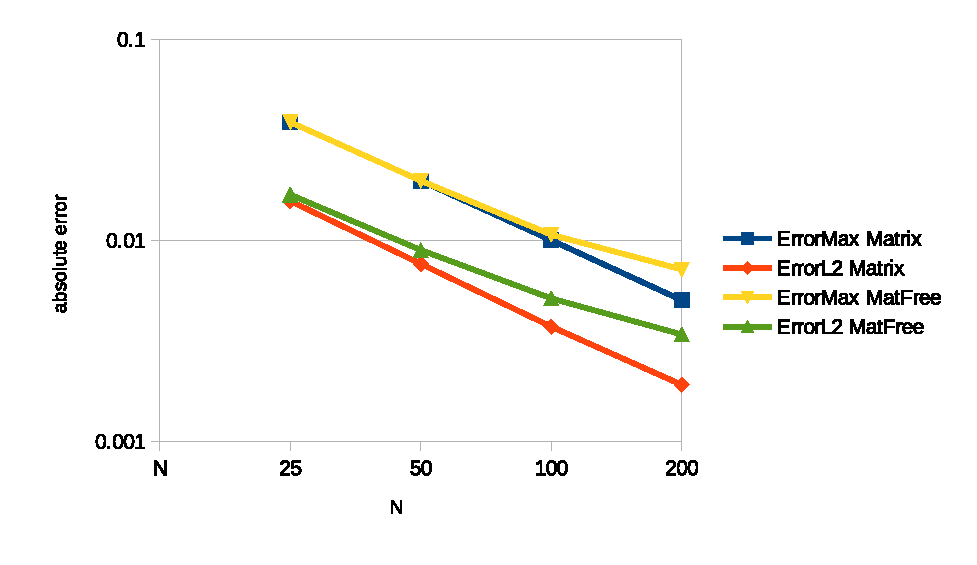
\includegraphics[width=\linewidth]{figs/errorbeta4}
		\caption{$\beta_1=0.4$}
	\end{subfigure}
	\begin{subfigure}{.6\linewidth}
		\includegraphics[width=\linewidth]{figs/errorbeta8}
		\caption{$\beta_2=0.4$}
	\end{subfigure}
	\caption{Scherk's surface on a truncated domain for different choices of the scaling factor $\beta$}\label{fig:conscherks}
\end{figure}

From figure~\ref{fig:conscherks} we can deduce, that for small enough $\beta$ and thus well enough behaved boundary functions, we get roughly first order of convergence in the error.

\newpage
\subsection{Sine boundaries}
The second testcase implemented uses $g|_{\text{bottom}}=g|_{\text{top}}=\sin(\pi(x-0.5))$ and $g|_{\text{left}}=g|_{\text{right}}=\sin(\pi(y-0.5))$.
By running a simulation with standard parameters (standard \texttt{params.in}-file), we get the surface in figure~\ref{fig:sine}.
\begin{figure}
	\begin{subfigure}{.49\linewidth}
		\centering
		\includegraphics[width=\linewidth]{figs/sine}
		\caption{Sine-testcase}\label{fig:sine}
	\end{subfigure}
	\hfill
	\begin{subfigure}{.49\linewidth}
		\centering
		\includegraphics[width=\linewidth]{figs/piecewise}
		\caption{Piece-wise boundary conditions introduced in section~\ref{sec:pcs}. The boundary \texttt{bottom} is here on the left side, \texttt{top} being on the right.}\label{fig:pcs}
	\end{subfigure}
	\caption{Visualization of surfaces obtained by a specific choice piece-wise boundary conditions}
\end{figure}



\subsection{Piece-wise boundary conditions}\label{sec:pcs}
Furthermore, our \texttt{inputParser} using a modified ATMSP-library is able to parse piece-wise defined boundary conditions.
To contrive this, we implemented a kind of indicator functions, defined as $\textsf{smaller1}(x): \mathbb{R} \to \{0,1\}, \textsf{larger1}(x): \mathbb{R} \to \{0,1\}$
\begin{equation}
	\textsf{smaller1}(x) = \begin{cases}
	1&, \text{ if } x \le 1 \\ 0&, \text{ else } 
	\end{cases}, \quad 	\textsf{larger1}(x) = \begin{cases}
	1&, \text{ if } x \ge 1 \\ 0&, \text{ else } 
	\end{cases} 
\end{equation}
Using these two functions, while scaling $x$ on the interval one wishes to constrain on, it is able to parse piece-wise defined functions. 

As an example, we chose the following: On the left and right boundary, $g|_{\text{left}}= g|_{\text{right}}=0$, while on the upper (top) boundary, we choose a two lines, meeting continuously in the middle above 0, on the lower (bottom) boundary, they are mirrored along the $x,y$ plane, and meet below 0 (this is not smooth, but will also yield a valid surface).

The result can be found in figure~\ref{fig:pcs}.


\newpage
\subsection{Interpretation of convergence results}
At last, we investigate the convergence behaviour of the different Jacobians implemented. Since adjoint AD by hand and symbolic differentiation basically correspond to each other, we only depict the former here. 

It can be easily seen, that the matrix-free algorithm needs much less Newton iterations to converge. The reason therefore lies in the fact, that we cannot directly compare one matrix-free Newton iteration with one iteration of the algorithms assembling a matrix. The latter linearize the MSE once per Newton iteration, and then solve for the update step. The former basically builds a new linearization within each step of the underlying linear systems algorithms, since the action of the Jacobian is always considered on the updated solution. This results in less iterations needed, while considering the run-time (section~\ref{sec:tim})
While the matrix-free method converge approximately in second order, the matrix-assembling methods are approximately first order. Also, one can see, that the matrix-free convergence follows a non-linear curve, in contrast to using a matrix-depending algorithm.


Apart from that, we observe, that for both methods, the hierarchy of the convergence per testcase ($\leftrightarrow$ boundary condition) is the same. The slowest convergence is obtained by Scherk's surface with a large scaling factor $\beta=0.8$, which is expected from our findings in section~\ref{sec:scherkolm}. The nicest/smoothest boundary is given by Scherk's surface with $\beta=0.4$, resulting in the fastest convergence. Both the sine-boundaries as well as our piece-wise initial condition do have a few non-smooth points (the sine on the edges, the piece-wise on the \texttt{bottom} and \texttt{top}-boundary), and thus have comparable convergence. 
Given the fact, that the order of convergence is quite similar for all testcases, we can conclude, that the number of iterations depends significantly on the initial residual. Typically, the residual decreases monotonically, though for some testcases, there is a short increase in the beginning. This might be improved by decreasing the relaxation parameter in the input file.

\begin{figure}
	\centering
	\begin{subfigure}{\linewidth}
		\centering
		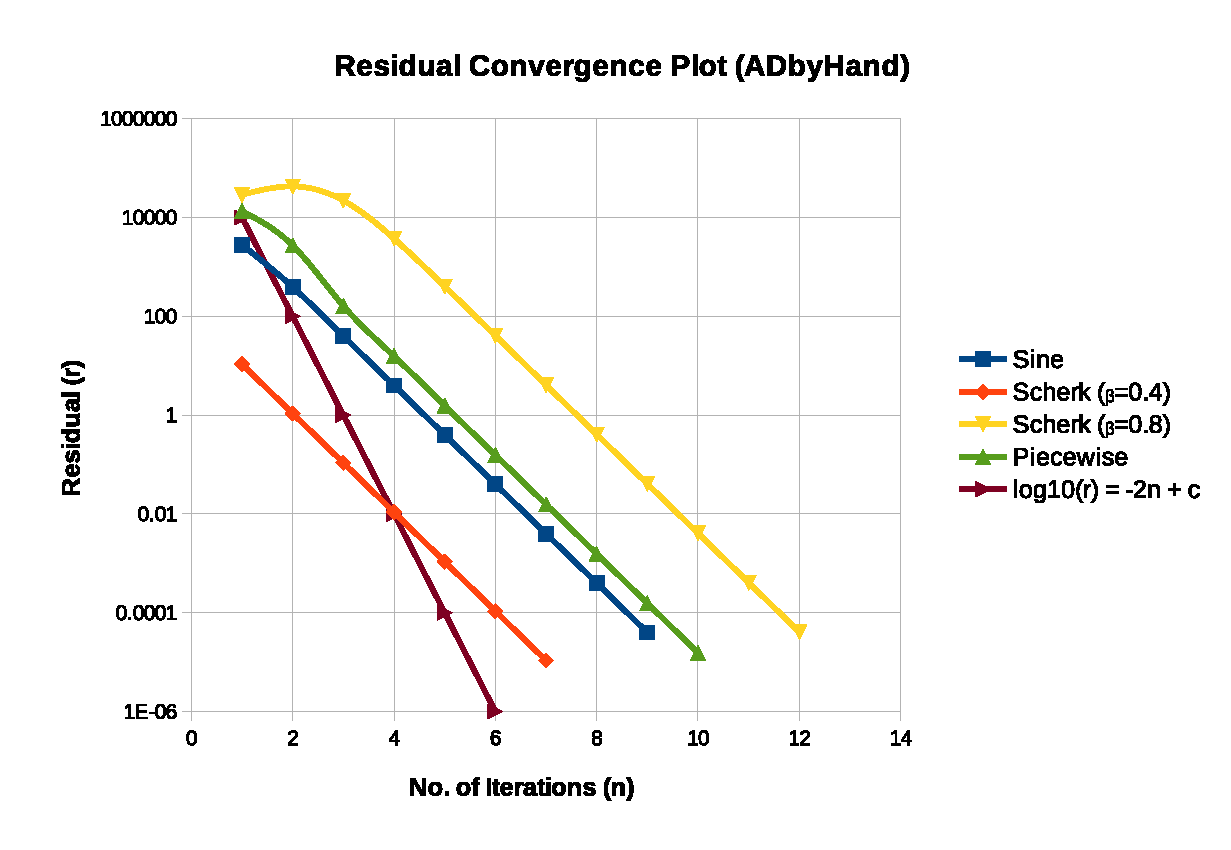
\includegraphics[width=\linewidth]{figs/ADbyHand}
		\caption{Jacobian by AD by hand (equivalent to symbolic)}
	\end{subfigure}
	\hfill
	\begin{subfigure}{\linewidth}
		\centering
		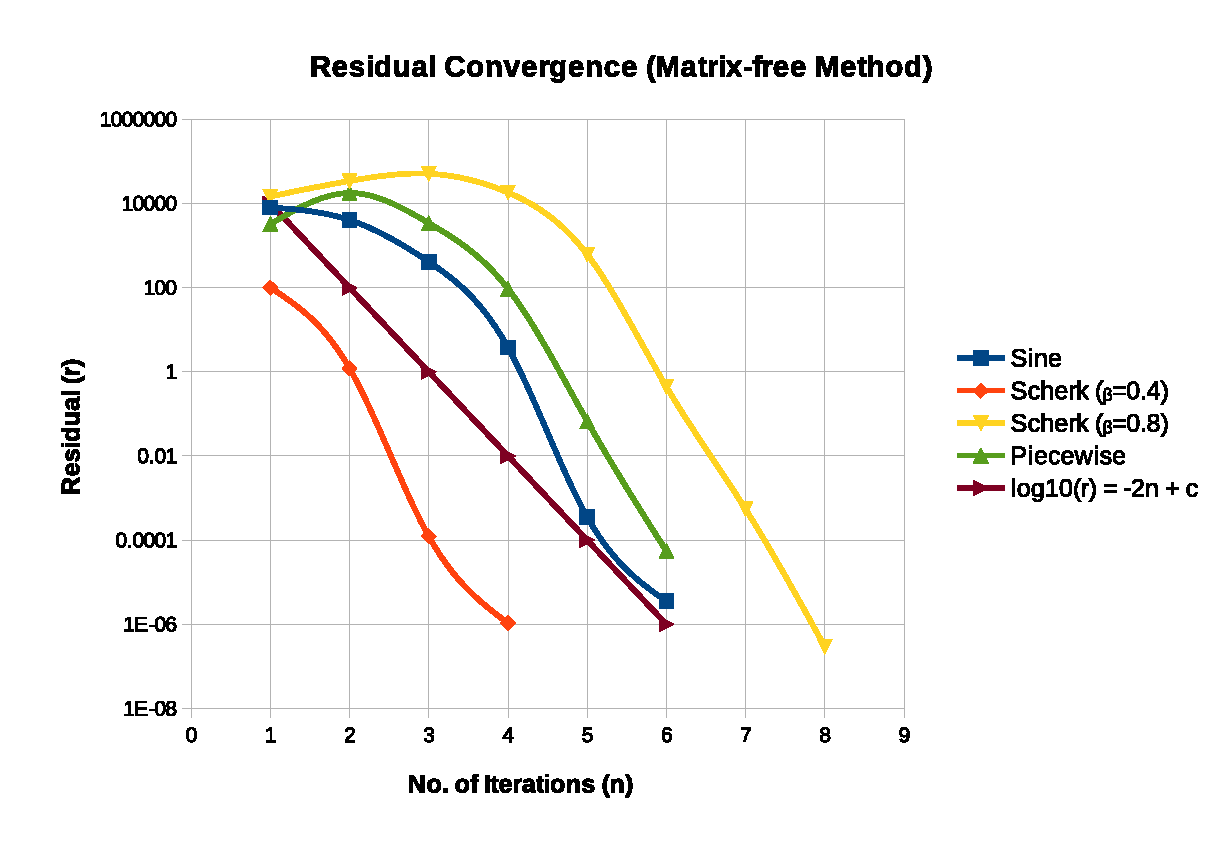
\includegraphics[width=\linewidth]{figs/Matrixfree}
		\caption{Matrix-free Jacobian}
	\end{subfigure}
	\caption{Convergence results for the residual $\lVert r_k \rVert _2= \lVert \mSurfDisc{z^h_k}\rVert_2$ depending on different choices of the right-hand-side; all using the solution of the Laplace equation as a initial guess}%; All methods use $\textsc{TOL_\text{linsolver}}=10^{-7}$, which is small enough for the matrix-free algorithm to converge properly.}
\end{figure}

Furthermore, tests revealed, that the Laplace initial guess greatly improved convergence with respect to the other two options (since it decreases the initial residual by pre-shaping the curvature), and in some cases, is required to converge at all. We do not present the results here.


\clearpage
\subsection{Timings}\label{sec:tim}

\begin{figure}[H]
	\centering
	\begin{subfigure}[b]{0.48\linewidth}
		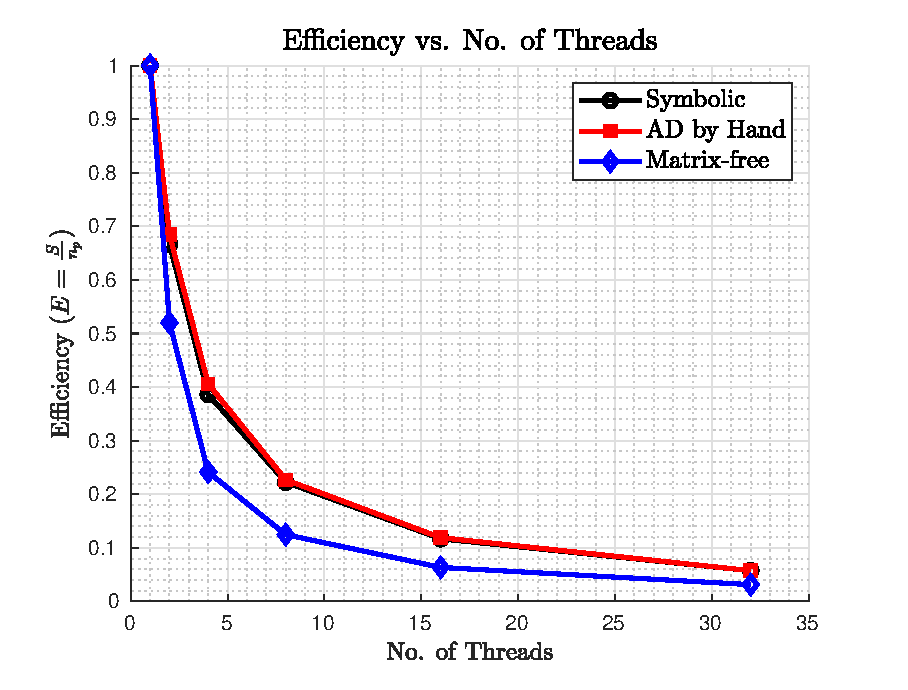
\includegraphics[width=\linewidth]{./figs/efficiency.eps}
	\end{subfigure}
	\begin{subfigure}[b]{0.48\linewidth}
		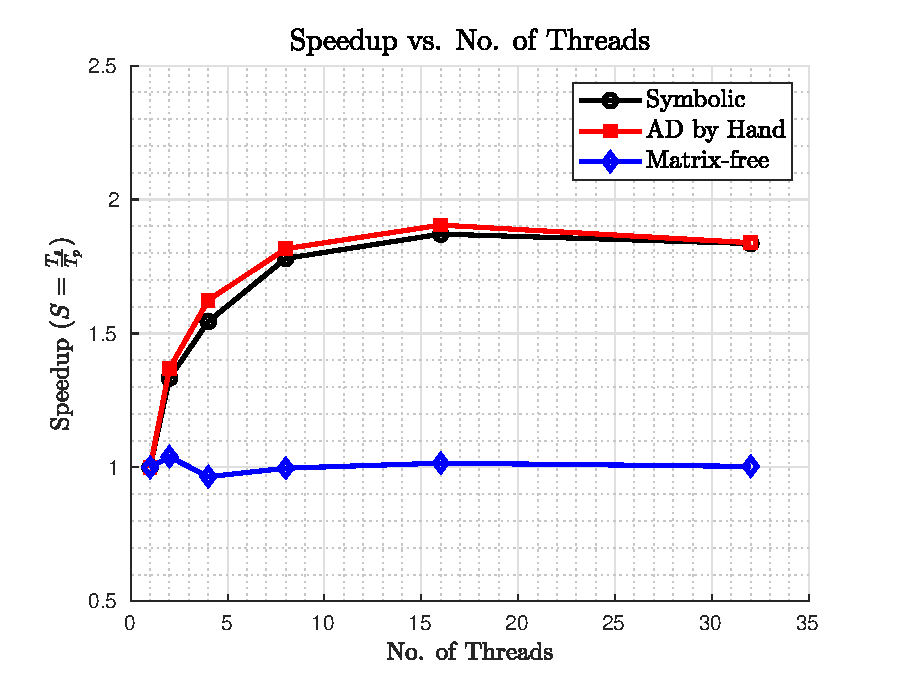
\includegraphics[width=\linewidth]{./figs/speedup.eps}
	\end{subfigure}
	\caption{Parallel Efficiency and Speedup plots for different Jacobian methods}\label{fig: Timing}
\end{figure}

The code was timed to check the efficiency of the OpenMP parallelization. It can be seen, that for N = 1000, both Symbolic and AD by Hand take up as much time as the Matrix-free method for N = 500. Although the Matrix-free method takes more time per iteration, it requires fewer iterations to converge as when compared to the other two methods.
This can be asserted mainly due the fact that every Newton iteration of the matrix-free algorithm calls $\texttt{dco}$ a large number of times (\# iterations for the linear solve), and each \texttt{dco}-call is costly. On the other hand, this has the effect, that less Newton iterations are needed in general, since every Newton iteration effectively uses a new linearization of the Jacobian for each iteration of the linear solver.

As an example set, for N=500, tolerance for the residual inside the Newton iterations 10$^{-6}$ and linear solver tolerance as 10$^{-7}$ , we get the time for the execution of the code as 279.220 [s] on average, while we use Newton's tolerance as 10$^{-3}$ and linear solver tolerance as 10$^{-7}$, the execution time is 155.364 [s]. This is approximately half of the time compared to the previous case. For both these cases, we get the same error measured in both $\ell_2$-norm and $\max$-norm.

\newpage
% #########################################################################
\section{Conclusion and outlook}
This last section should summarize the conclusions that we were able to draw from working on this project, and provides a short outlook on what could be still done to improve the software.

The main take-away messages, we were able to draw from the project, are:
\begin{itemize}
	\item We were given the chance, to build a numerical software from scratch. This essentially forced us, to mobilize knowledge from most of the (mandatory) courses so far the Simulation Sciences curriculum. This way we saw, that we are already able to apply the theory from our studies (in some extent) to a toy problem (that could easily be extended to a practical one).
	\item The complexity of the project, though moderate, but fitted in a quite narrow time-frame required a good project management amongst the group, in case one wanted to implement everything, that was required. We learnt to appreciate platforms for digital collaboration, such as \texttt{git}, to realize working in a team on a software project.
\end{itemize}

Although our code fulfils the minimum requirements, there are a few points, that could be improved, and give rise to an outlook, what could be done in a second iteration:
\begin{itemize}
	\item {The code could be modified to better suit for testing purposes. Some test methods were not ethically called due to private dependencies. Appropriate return functions would make it easier and simpler.}
	\item {Private methods could be tested by yet another way: inclusion of \texttt{Gtest\_prod.h} . Unfortunately, not supported by standard CMake.}
	\item {Extension of the minimal surface problem to include time varying boundary conditions to account for evolution of solution w.r.t. time}
	\item{Properly investigate the convergence behaviour of the method, and connect it to the smoothness of the boundary.}
	\item{Development of a more flexible grid, that allows (i) piece-wise boundary condition, that rely not on a parser, but on flexibly choosable boundary sections. I might furthermore be extended to arbitrary geometries, which requires a proper meshing algorithm, and different shapes of the elements. This would be simplified substantially then if one would use Finite Elements for the discretization.}
\end{itemize}

% #########################################################################

%
\bibliographystyle{apalike}
\bibliography{bibliography}
\clearpage
\appendix
\section{User manual}
\small
This section provides a short description on how to run the code. The software accompanying this report is self-contained and made to run on the RWTH cluster.\footnote{using either the current versions of the Intel (19) or GCC (9) compiler.}

\color{@darkred}
\emph{Update as of last week of February:} During the last week of February, the following options became necessary for the code to compile. As of February 28, it works again without, but if not, load the following options:

\lstset{backgroundcolor=\color{gray!20}, language=bash, basicstyle=\ttfamily \small, }
\begin{lstlisting}
module switch intel gcc 
module load LIBRARIES
module load intelmkl    
\end{lstlisting}
\normalcolor

\subsection{Compilation}
To compile the code, open a terminal inside \texttt{source/}. 
\lstset{backgroundcolor=\color{gray!20}, language=bash, basicstyle=\ttfamily \small}
\begin{lstlisting}
	cd build 
	cmake .. 
	make
\end{lstlisting}
The standard setup is the CMAKE compile option \texttt{Release} admitting some compiler optimization. If some additional debug information is desired, change the option to \texttt{debug} inside \texttt{CMakeLists.txt}.
\subsection{Running a simulation}
To run a simulation, go to the folder testcases or create a new folder with a valid \texttt{params.in}-file.

Inside this \texttt{params.in}-file, one can find the options to set with descriptions.

\noindent To run the a simulation, execute the following, once the input file is set up:
\lstset{backgroundcolor=\color{gray!20}, language=bash, basicstyle=\ttfamily \small, breaklines=true}
\begin{lstlisting}
	cd <folder with params.in> 
	export NAG_KUSARI_FILE=<path to nag_key.txt>              # needed if jacobianOpt=2 
	ln -s <path to executable minSurf in build/> .            # symbolic link for convenient execution 
	./minSurf
\end{lstlisting}
Now, the resulting output can be inspected by opening the \texttt{.vts}-files inside \texttt{surfaces/} using Paraview\footnote{to use this on the cluster, execute \texttt{module load GRAPHICS paraview} beforehand.}. If one is interesting in the convergence, one can find the residual data over iteration inside \texttt{residual/}, which can be also plotted using Paraview. 

\normalsize
\end{document}          
